%\documentclass[]{beamer}
\documentclass[handout]{beamer}
%\usepackage[dvips]{color}
\usepackage{graphicx}
\usepackage{amsmath,amssymb,array,comment,eucal}
\newcommand{\e}{\mathbf{e}}
\renewcommand{\P}{\mathbf{P}}
\newcommand{\F}{\mathbf{F}}
\newcommand{\R}{\textsf{R}}
\newcommand{\mat}[1] {\mathbf{#1}}
%\newcommand{\ind}{\mathrel{\mathop{\sim}\limits^{\mathit{ind}}}}
%\newcommand{\iid}{\mathrel{\mathop{\sim}\limits^{\mathit{iid}}}}
\newcommand{\E}{\textsf{E}}
\newcommand{\SE}{\textsf{SE}}
\newcommand{\SSE}{\textsf{SSE}}
\newcommand{\RSS}{\textsf{RSS}}
\newcommand{\FSS}{\textsf{FSS}}
\renewcommand{\SS}{\textsf{SS}}
\newcommand{\MSE}{\textsf{MSE}}
\newcommand{\SSR}{\textsf{SSR}}
\newcommand{\Be}{\textsf{Beta}}
\newcommand{\St}{\textsf{St}}
%\newcommand{\C}{\textsf{C}}
\newcommand{\GDP}{\textsf{GDP}}
\newcommand{\NcSt}{\textsf{NcSt}}
\newcommand{\Bin}{\textsf{Bin}}
\newcommand{\NB}{\textsf{NegBin}}
\renewcommand{\NG}{\textsf{NG}}
\newcommand{\N}{\textsf{N}}
\newcommand{\Ber}{\textsf{Ber}}
\newcommand{\Poi}{\text{Poi}}
\newcommand{\Gam}{\textsf{Gamma}}
\newcommand{\BB}{\textsf{BB}}
\newcommand{\Gm}{\textsf{G}}
\newcommand{\Un}{\textsf{Unif}}
\newcommand{\Ex}{\textsf{Exp}}
\newcommand{\DE}{\textsf{DE}}
\newcommand{\tr}{\textsf{tr}}
\newcommand{\cF}{{\cal{F}}}
\newcommand{\cL}{{\cal{L}}}
\newcommand{\cI}{{\cal{I}}}
\newcommand{\cB}{{\cal{B}}}
\newcommand{\cP}{{\cal{P}}}
\newcommand{\bbR}{\mathbb{R}}
\newcommand{\bbN}{\mathbb{N}}
\newcommand{\pperp}{\mathrel{{\rlap{$\,\perp$}\perp\,\,}}}
\newcommand{\OFP}{(\Omega,\cF, \P)}
\newcommand{\eps}{\boldsymbol{\epsilon}}
\newcommand{\1}{\mathbf{1}_n}
\newcommand{\gap}{\vspace{8mm}}
\newcommand{\ind}{\mathrel{\mathop{\sim}\limits^{\rm ind}}}
\newcommand{\simiid}{\ensuremath{\mathrel{\mathop{\sim}\limits^{\rm
iid}}}}
\newcommand{\eqindis}{\ensuremath{\mathrel{\mathop{=}\limits^{\rm D}}}}
\newcommand{\iid}{\textit{i.i.d.}}
\newcommand{\SSZ}{S_{zz}}
\newcommand{\SZW}{S_{zw}}
\newcommand{\Var}{\textsf{Var}}
\newcommand{\corr}{\textsf{corr}}
\newcommand{\diag}{\textsf{diag}}
\newcommand{\var}{\textsf{var}}
\newcommand{\Cov}{\textsf{Cov}}
\newcommand{\Sam}{{\cal S}}
\def\H{\mathbf{H}}
\newcommand{\I}{\mathbf{I}}
\newcommand{\Y}{\mathbf{Y}}
\newcommand{\tY}{\tilde{\mathbf{Y}}}
\newcommand{\Yhat}{\hat{\mathbf{Y}}}
\newcommand{\Yobs}{\mathbf{Y}_{{\cal S}}}
\newcommand{\barYobs}{\bar{Y}_{{\cal S}}}
\newcommand{\barYmiss}{\bar{Y}_{{\cal S}^c}}
\def\bv{\mathbf{b}}
\def\X{\mathbf{X}}
\def\tX{\tilde{\mathbf{X}}}
\def\x{\mathbf{x}}
\def\xbar{\bar{\mathbf{x}}}
\def\Xbar{\bar{\mathbf{X}}}
\def\Xg{\mathbf{X}_{\boldsymbol{\gamma}}}
\def\Ybar{\bar{\Y}}
\def\ybar{\bar{y}}
\def\y{\mathbf{y}}
\def\Yf{\mathbf{Y_f}}
\def\W{\mathbf{W}}
\def\L{\mathbf{L}}
\def\w{\mathbf{w}}
\def\U{\mathbf{U}}
\def\V{\mathbf{V}}
\def\Q{\mathbf{Q}}
\def\Z{\mathbf{Z}}
\def\z{\mathbf{z}}
\def\v{\mathbf{v}}
\def\u{\mathbf{u}}

\def\zero{\mathbf{0}}
\def\one{\mathbf{1}}
\newcommand{\taub}{\boldsymbol{\tau}}
\newcommand{\betav}{\boldsymbol{\beta}}
\newcommand{\alphav}{\boldsymbol{\alpha}}
\newcommand{\A}{\mathbf{A}}
\def\a{\mathbf{a}}
\def\K{\mathbf{K}}
\newcommand{\B}{\mathbf{B}}
\def\b{\boldsymbol{\beta}}
\def\bhat{\hat{\boldsymbol{\beta}}}
\def\btilde{\tilde{\boldsymbol{\beta}}}
\def\tb{\tilde{\boldsymbol{\beta}}}
\def\bg{\boldsymbol{\beta_\gamma}}
\def\bgnot{\boldsymbol{\beta_{(-\gamma)}}}
\def\mub{\boldsymbol{\mu}}
\def\tmub{\tilde{\boldsymbol{\mu}}}
\def\muhat{\hat{\boldsymbol{\mu}}}
\def\t{\boldsymbol{\theta}}
\def\tk{\boldsymbol{\theta}_k}
\def\tj{\boldsymbol{\theta}_j}
\def\Mk{\boldsymbol{{\cal M}}_k}
\def\M{\boldsymbol{{\cal M}}}
\def\Mj{\boldsymbol{{\cal M}}_j}
\def\Mi{\boldsymbol{{\cal M}}_i}
\def\Mg{{\boldsymbol{{\cal M}_\gamma}}}
\def\Mnull{\boldsymbol{{\cal M}}_{N}}
\def\gMPM{\boldsymbol{\gamma}_{\text{MPM}}}
\def\gHPM{\boldsymbol{\gamma}_{\text{HPM}}}
\def\Mfull{\boldsymbol{{\cal M}}_{F}}
\def\tg{\boldsymbol{\theta}_{\boldsymbol{\gamma}}}
\def\g{\boldsymbol{\gamma}}
\def\eg{\boldsymbol{\eta}_{\boldsymbol{\gamma}}}
\def\G{\mathbf{G}}
\def\cM{\cal M}
\def\D{\Delta}
\def \shat{{\hat{\sigma}}^2}
\def\uv{\mathbf{u}}
\def\l {\lambda}
\def\d{\delta}
\def\Sigmab{\boldsymbol{\Sigma}}
\def\Lambdab{\boldsymbol{\Lambda}}
\def\lambdab{\boldsymbol{\lambda}}
\def\Mg{{\cal M}_\gamma}
\def\S{{\cal{S}}}
\def\qg{p_{\boldsymbol{\gamma}}}
\def\pg{p_{\boldsymbol{\gamma}}}
\def\t{\boldsymbol{\theta}}  
\def\T{\boldsymbol{\Theta}}  
\usepackage{verbatim}

\usetheme{Warsaw}
\title{Distribution Assumptions}
\subtitle{Merlise Clyde}
\author{STA721 Linear Models}
\institute{Duke University}
\date{\today}
\logo{duke.eps}

\begin{document}
\maketitle

\begin{frame}\frametitle{Outline}
Topics
  \begin{itemize}
  \item Normality \& Transformations
  \item Box-Cox
  \item Nonlinear Regression
  \end{itemize}


Readings: Christensen  Chapter 13  \& Wakefield Chapter 6
\end{frame}
%\section{Models}
\begin{frame} \frametitle{ Linear Model}
Linear Model again:
 $$ \Y = \mub + \eps $$ \pause
Assumptions: \pause
\begin{eqnarray*}
   \mub \in C(\X) & \Leftrightarrow & \mub = \X \b \pause \\
   \eps  & \sim &  \N(\zero_n, \sigma^2 \I_n) \pause
\end{eqnarray*}
\begin{itemize}
\item Normal Distribution for $\eps$ with constant variance \\
\item Outlier Models
\item Robustify with heavy tailed error distributions
\item Computational Advantages of Normal Models
\end{itemize}
\end{frame}


\begin{frame}
    \frametitle{Normality}
    Recall
    \begin{eqnarray*}
 \e & = &(\I - \P_\X) \Y \pause \\      
 & = & (\I - \P_\X)(\X \bhat + \eps)  \pause\\
 & = &  (\I - \P_\X)\eps  \pause
    \end{eqnarray*}
$$e_i = \epsilon_i - \sum_{j=1}^n h_{ij} \epsilon_j$$  \pause
Lyapunov CLT implies that  residuals will be approximately normal
(even for modest $n$), 
if the errors are not normal  \pause

\vfill

``Supernormality of residuals''
  \end{frame}
  \begin{frame}
    \frametitle{Q-Q Plots}
\begin{itemize}
\item Order $e_i$: $e_{(1)} \le e_{(2)} \ldots \le e_{(n)}$  sample
    order statistics or sample quantiles  \pause
\item Let $z_{(1)} \le z_{(2)} \ldots z_{(n)}$ denote the expected
  order statistics of a sample of size $n$ from a standard normal
  distribution ``theoretical quantiles''  \pause
\item If the $e_i$ are normal then $\E[e_{(i)}] = \sigma z_{(i)}$   \pause
\item Expect that points in a scatter plot of $e_{(i)}$ and $z_{(i)}$
  should be on a straight line.  \pause
\item Judgment call - use simulations to gain experience!
\end{itemize}
    
  \end{frame}

  \begin{frame}
    \frametitle{Animal Example}

\centerline{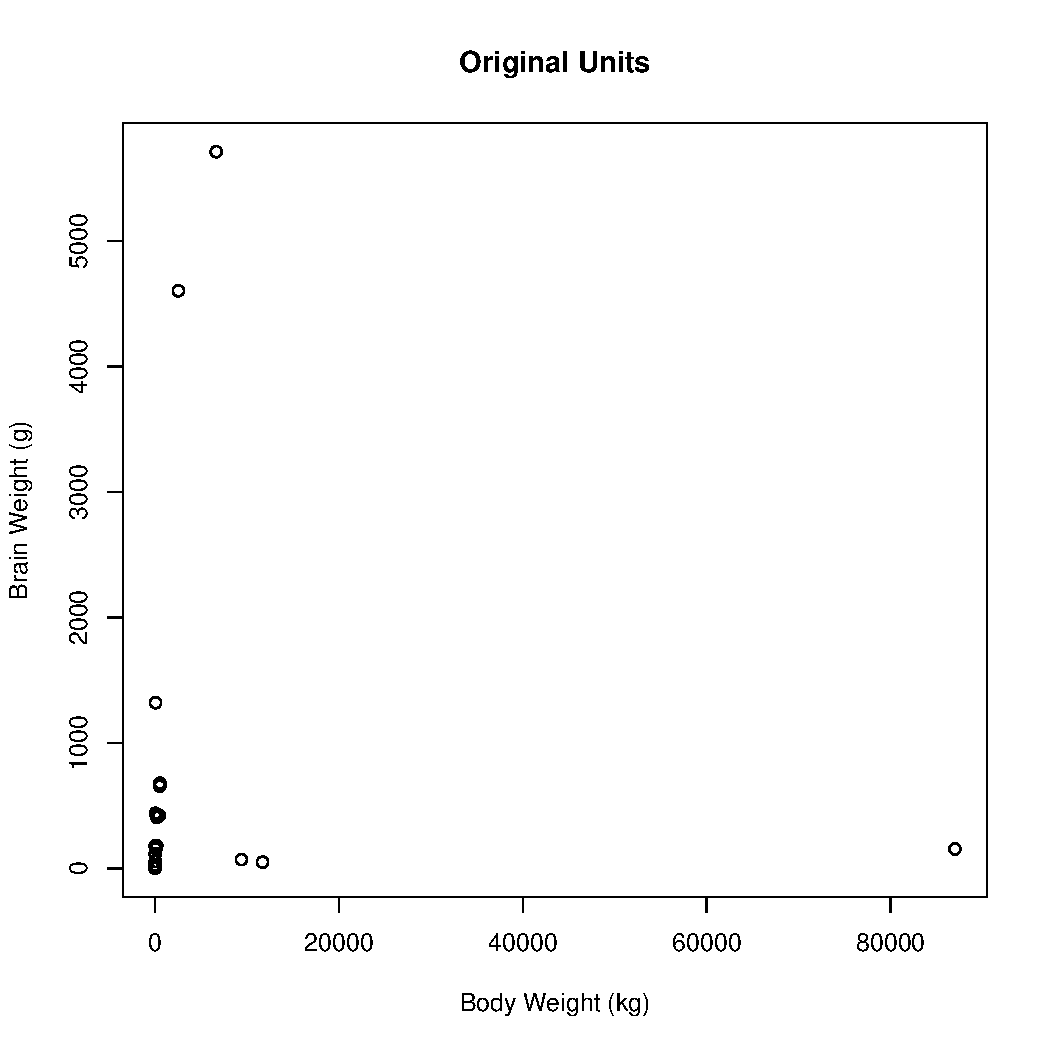
\includegraphics[height=3in]{brain}}
  \end{frame}

  \begin{frame}
    \frametitle{Residual Plots}

\centerline{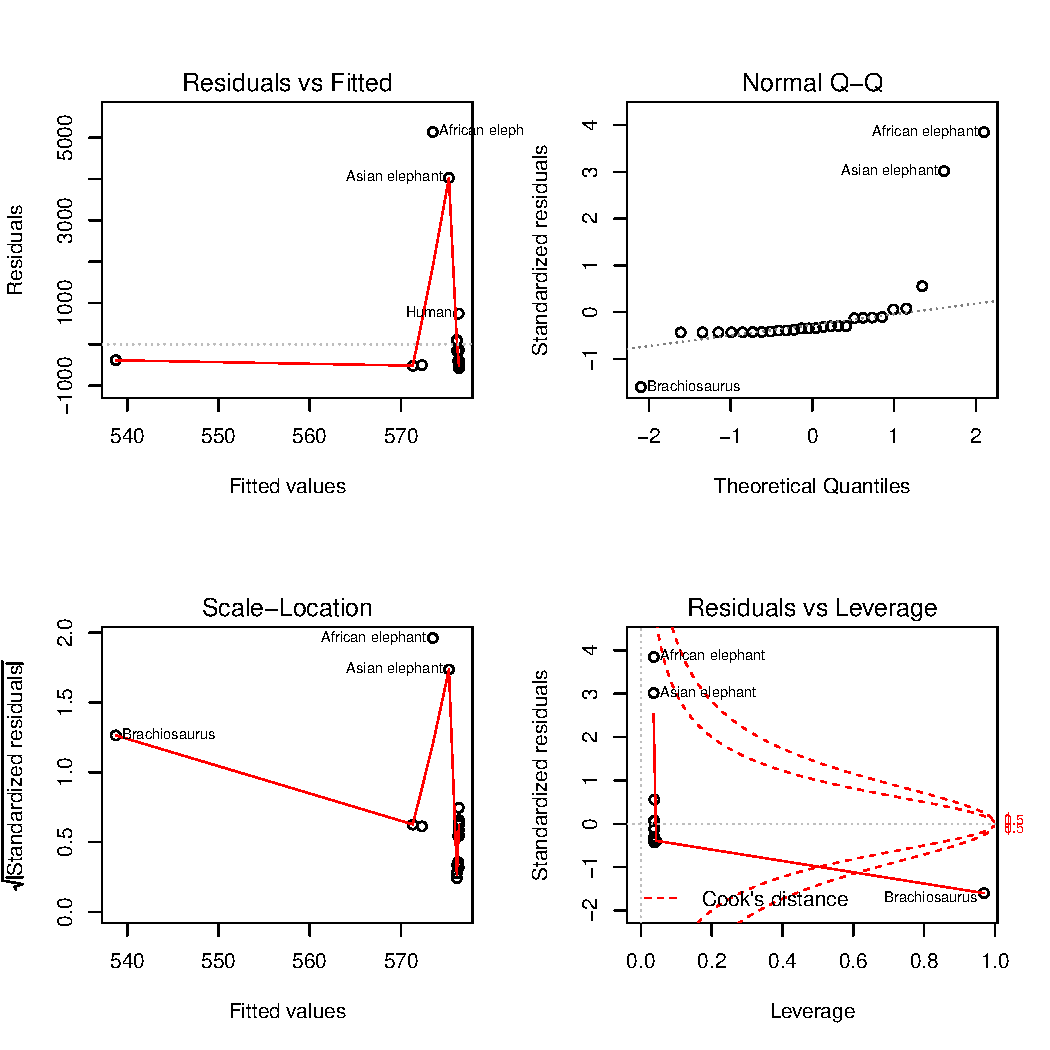
\includegraphics[height=3in]{brains-resid}}
  \end{frame}


  \begin{frame}
    \frametitle{Box-Cox Transformation}
    Box and Cox (1964) suggested a family of power transformations for
    $Y > 0$  \pause
$$
U(\Y, \lambda) =  Y^{(\lambda)} = \left\{
   \begin{array}{ll}
     \frac{(Y^\lambda -1)}{\lambda} & \lambda \neq 0 \\
 \log(Y) & \lambda = 0
   \end{array} \right.
$$  \pause

\begin{itemize}
\item Estimate $\lambda$ by maximum Likelihood  \pause
$$\cL(\lambda, \b, \sigma^2) \propto \prod f(y_i \mid \lambda, \b,
\sigma^2)$$

\item  $U(\Y, \lambda) = Y^{(\lambda)} \sim \N(\X\b, \sigma^2)$
  \pause
\item Jacobian term is $\prod_i y_i^{\lambda - 1}$ for all $\lambda$  \pause
\item Profile Likelihood based on substituting MLE $\b$ and $\sigma^2$
  for each value of $\lambda$ is 
$$\log(\cL(\lambda) \propto (\lambda -1)
\sum_i \log(Y_i) - \frac{n}{2} \log(\SSE (\lambda))$$
\end{itemize}

  \end{frame}
  \begin{frame}
    \frametitle{ Profile Likelihood}

\centerline{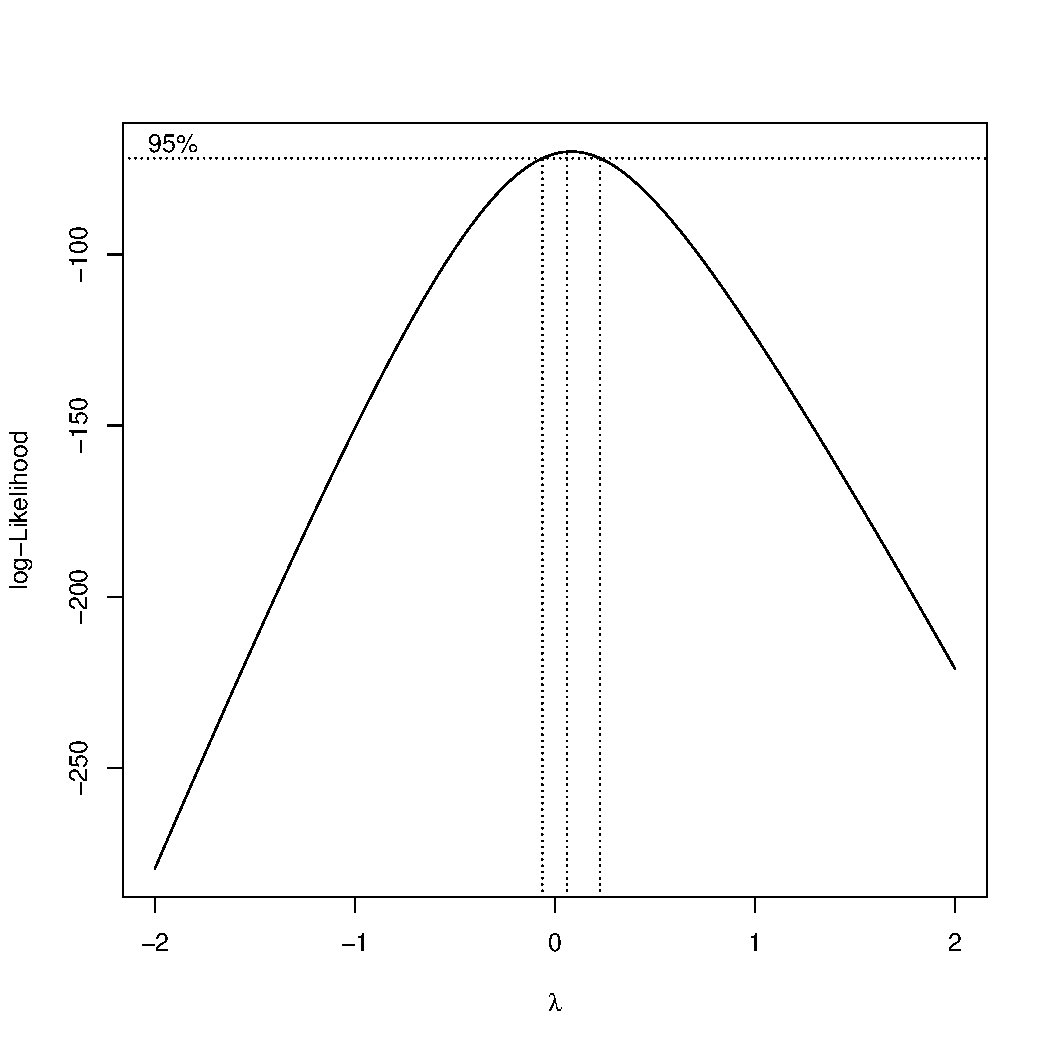
\includegraphics[height=3in]{brains-BC}}
  \end{frame}

  \begin{frame}
    \frametitle{ Residuals After Transformation of Response}

\centerline{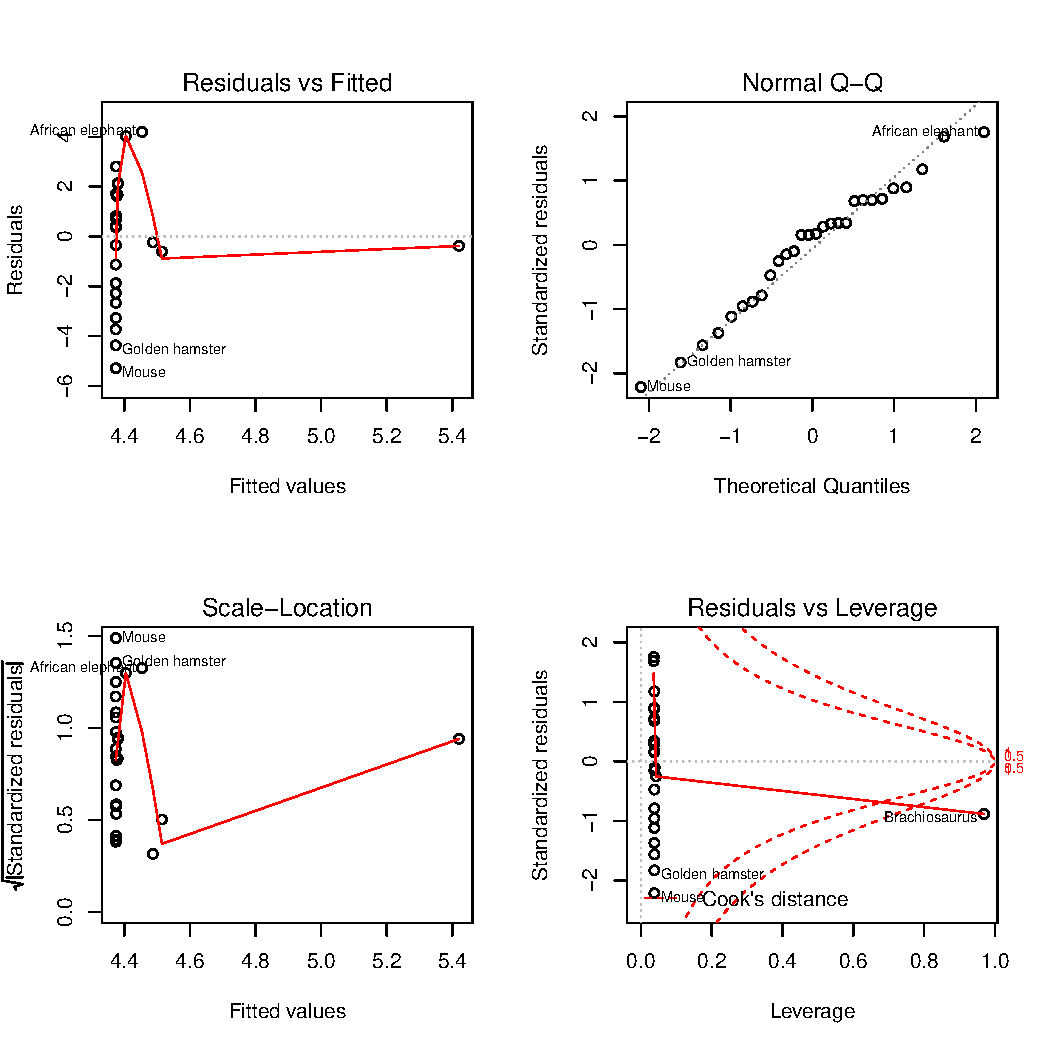
\includegraphics[height=3in]{brain-resid-logY}}

  \end{frame}
  \begin{frame}
    \frametitle{ Residuals After Transformation of Both}

\centerline{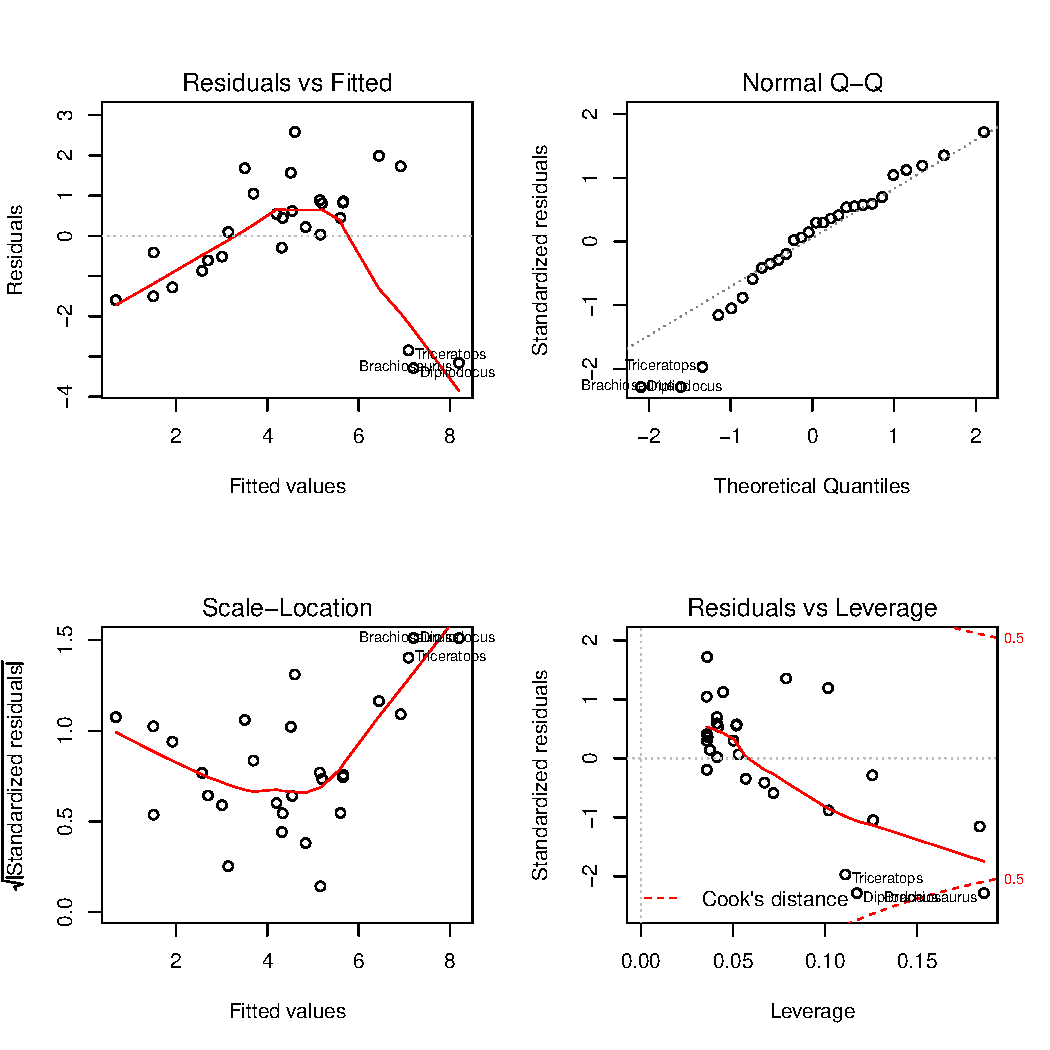
\includegraphics[height=3in]{brains-tran}}

  \end{frame}

 \begin{frame}
    \frametitle{ Transformed Data}

\centerline{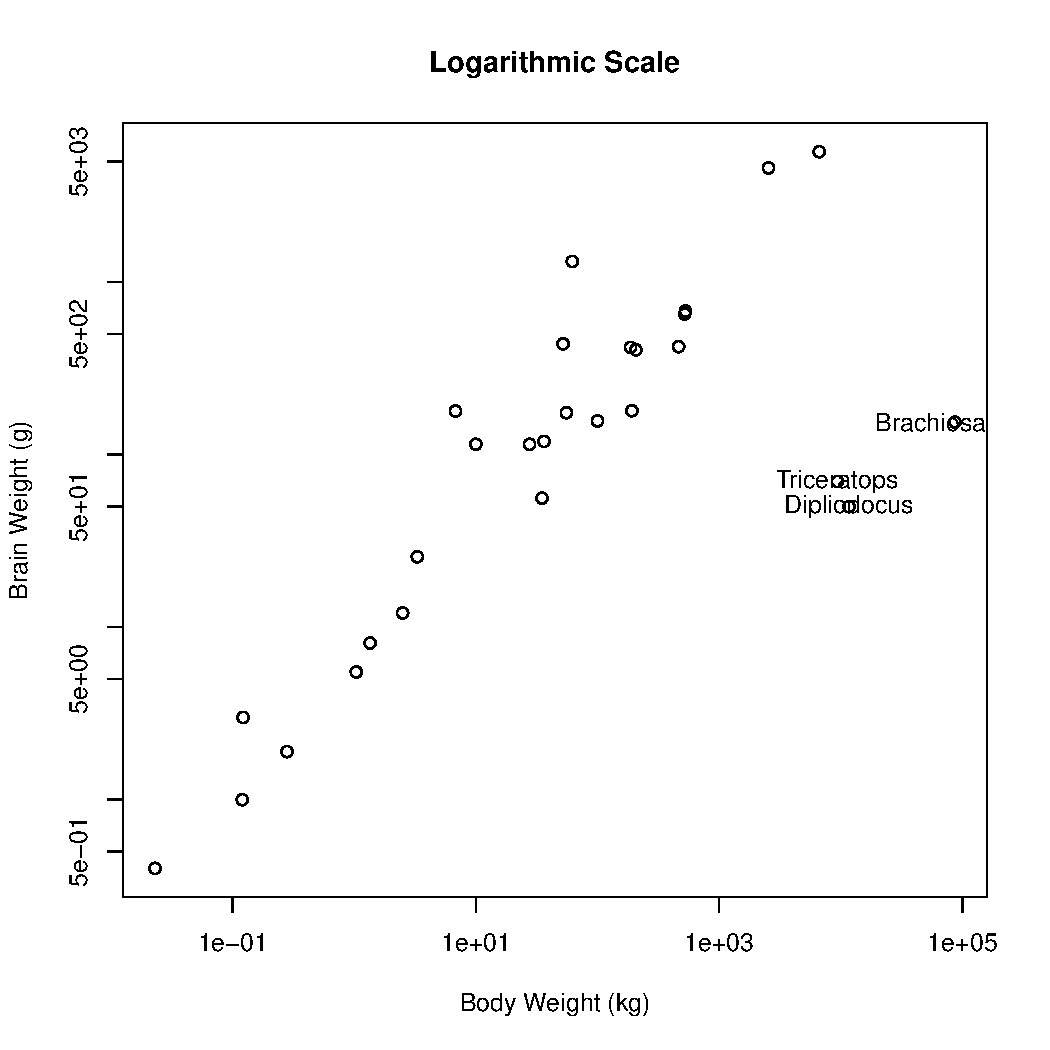
\includegraphics[height=3in]{brain-log}}

  \end{frame}

  \begin{frame}
    \frametitle{Test that Dinos are Outliers}
    \begin{table}[ht]
\begin{center}
\begin{tabular}{lrrrrrr}
  \hline
 & Res.Df & RSS & Df & Sum of Sq & F & Pr($>$F) \\ 
  \hline
1 & 23 & 12.12 &  &  &  &  \\ 
  2 & 26 & 60.99 & -3 & -48.87 & 30.92 & 0.0000 \\ 
   \hline
\end{tabular}
\end{center}
\pause
\begin{table}[ht]
\begin{center}
\begin{tabular}{rrrrr}
  \hline
 & Estimate & Std. Error & t value & Pr($>$$|$t$|$) \\ 
  \hline
(Intercept) & 2.1504 & 0.2006 & 10.72 & 0.0000 \\ 
  log(body) & 0.7523 & 0.0457 & 16.45 & 0.0000 \\ 
  Triceratops & -4.7839 & 0.7913 & -6.05 & 0.0000 \\ 
  Brachiosaurus & -5.6662 & 0.8328 & -6.80 & 0.0000 \\ 
  Dipliodocus & -5.2851 & 0.7949 & -6.65 & 0.0000 \\ 
   \hline
\end{tabular}
\end{center}
\end{table}
\pause
Dinosaurs come from a different population from mammals
\end{table}
  \end{frame}
\begin{frame}[fragile]  \frametitle{Model Selection Priors}
\begin{verbatim}
brains.bas = bas.lm(log(brain) ~ log(body) + diag(28),
   data=Animals,  prior="hyper-g-n", a=3, 
   modelprior=beta.binomial(1,28), 
   method="MCMC", n.models=2^17, MCMC.it=2^18)
# check for convergence
plot(brains.bas$probne0, brains.bas$probs.MCMC)
\end{verbatim}
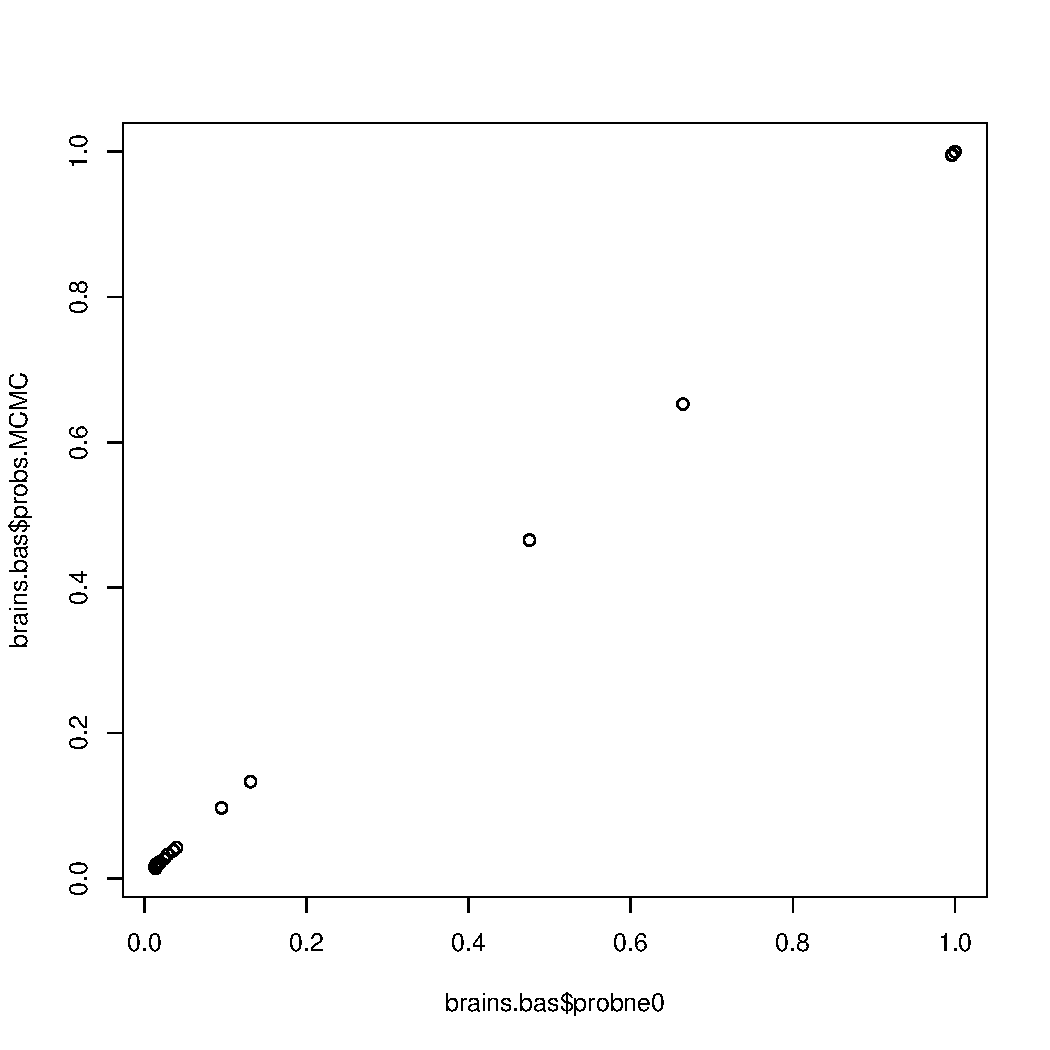
\includegraphics[height=2in]{bas-animals-conv}
\end{frame}

\begin{frame}  \frametitle{image(brains.bas)}
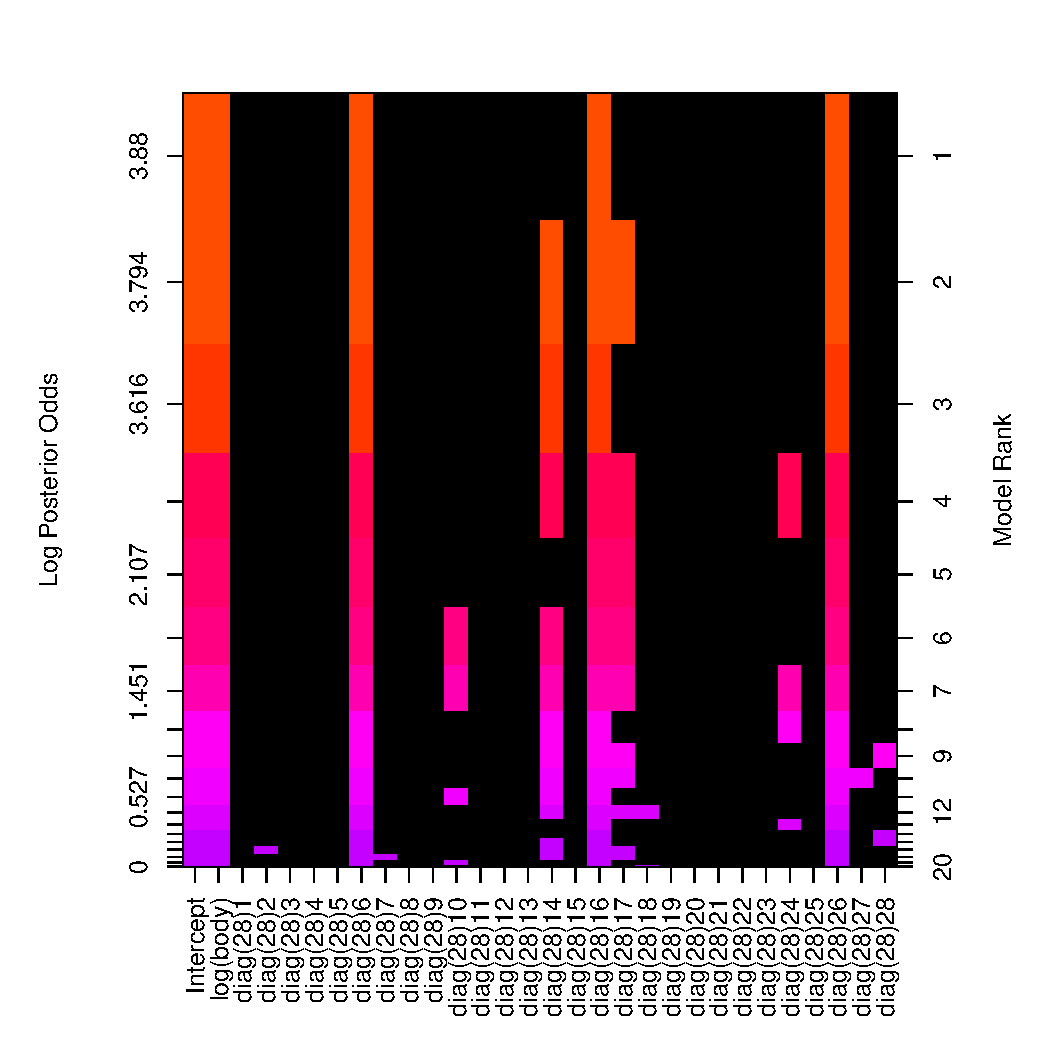
\includegraphics[height=2.75in]{brains-image}

{\tt rownames(Animals)[c(6, 14, 16, 26)]  }

{\tt "Dipliodocus" "Human" "Triceratops" "Brachiosaurus"}
\end{frame}

  \begin{frame}\frametitle{Variance Stabilizing Transformations}
    \begin{itemize}
    \item If $Y - \mu$ (approximately) $N(0, h(\mu))$ \pause
    \item Delta Method implies that 
$$g(Y) \stackrel{\cdot}{\sim}\N( g(\mu),  g'(\mu)^2 h(\mu)$$ 

\item Find function $g$ such that $g'(\mu)^2/h(\mu)$ is constant
$$g(Y) \sim N(g(\mu), c)$$
    \end{itemize}
  
\begin{itemize}
\item Poisson Counts ($Y > 3$): $g$ is square root transformation \pause
\item Binomial: arcsin($ \sqrt(Y)$)
\end{itemize}
Note: transformation for normality may not be the same as the variance
stabilizing transformation; boxcox assumes mean function is correct

\end{frame}

\begin{frame}{Nonlinear Models}
Drug concentration of caldralazine  at time $X_i$ in a cardiac
failure patient given a single 30mg dose  $(D = 30)$ given by \pause

$$
\mu(\b) = \left[\frac{D}{V} \exp(-\kappa_e x_i) \right]
$$
with $\b = (V, \kappa_e)$  $V = volume$ and $\kappa_e$ is the
elimination rate \pause
  
If $\log(Y_i)  = \log(\mu(\b)) + \epsilon_i$ with $\epsilon_i \simiid
N(0, \sigma^2)$ then the model is intrinisically linear (can transform
to linear model)
\begin{eqnarray*}
\log(\mu(\b)) & = & \log\left[\frac{D}{V} \exp(-\kappa_e x_i) \right]  \\
  & = & \log[D] - \log(V) -\kappa_e x_i \\
log(Y_i) - \log[30] & = &\beta_0 + \beta_1 x_i + \epsilon_i
\end{eqnarray*}
\pause

\end{frame}

\begin{frame}[fragile]\frametitle{Nonlinear Least Squares}
\begin{verbatim}
> conc.nlm = nls( log(y) ~ log((30/V)*exp(-k*x)), 
             data=df, start=list(V=vhat, k=khat))
> summary(conc.nlm)
Formula: log(y) ~ log((30/V) * exp(-k * x))
Parameters:
              Estimate Std. Error t value Pr(>|t|)    
V.(Intercept) 16.66331    7.11923   2.341 0.057796 .  
k.x            0.15211    0.02368   6.423 0.000673 ***

Residual standard error: 0.7411 on 6 degrees of freedom
Number of iterations to convergence: 0 
Achieved convergence tolerance: 3.978e-09
\end{verbatim}
\end{frame}


\begin{frame} {Additive Errors}
  \begin{itemize}
  \item  under  multiplicative log normal errors model is equivalent
    to linear model \pause
  \item with additive Gaussian errors (or other distributions) model
    is intrinsically nonlinear - nonlinear least squares (or posterior
    sampling) \pause
  \end{itemize}
$$ Y_i = (30/V) * exp(-k * x_i) + \epsilon_i$$ \pause
$$\epsilon_i \simiid \N(0, \sigma^2)$$ 
\end{frame}
\begin{frame}[fragile]\frametitle{Intrinsically Nonlinear Model}
\begin{verbatim}
> summary(conc.nlm)
Formula: y ~ (30/V) * exp(-k * x)
Parameters:
  Estimate Std. Error t value Pr(>|t|)    
V 13.06506    0.60899   21.45 6.69e-07 ***
k  0.18572    0.01124   16.52 3.14e-06 ***
---
Residual standard error: 0.05126 on 6 degrees of freedom
Number of iterations to convergence: 4 
Achieved convergence tolerance: 7.698e-06
\end{verbatim}
\end{frame}
\begin{frame} {Fitted Values \& Residuals}
  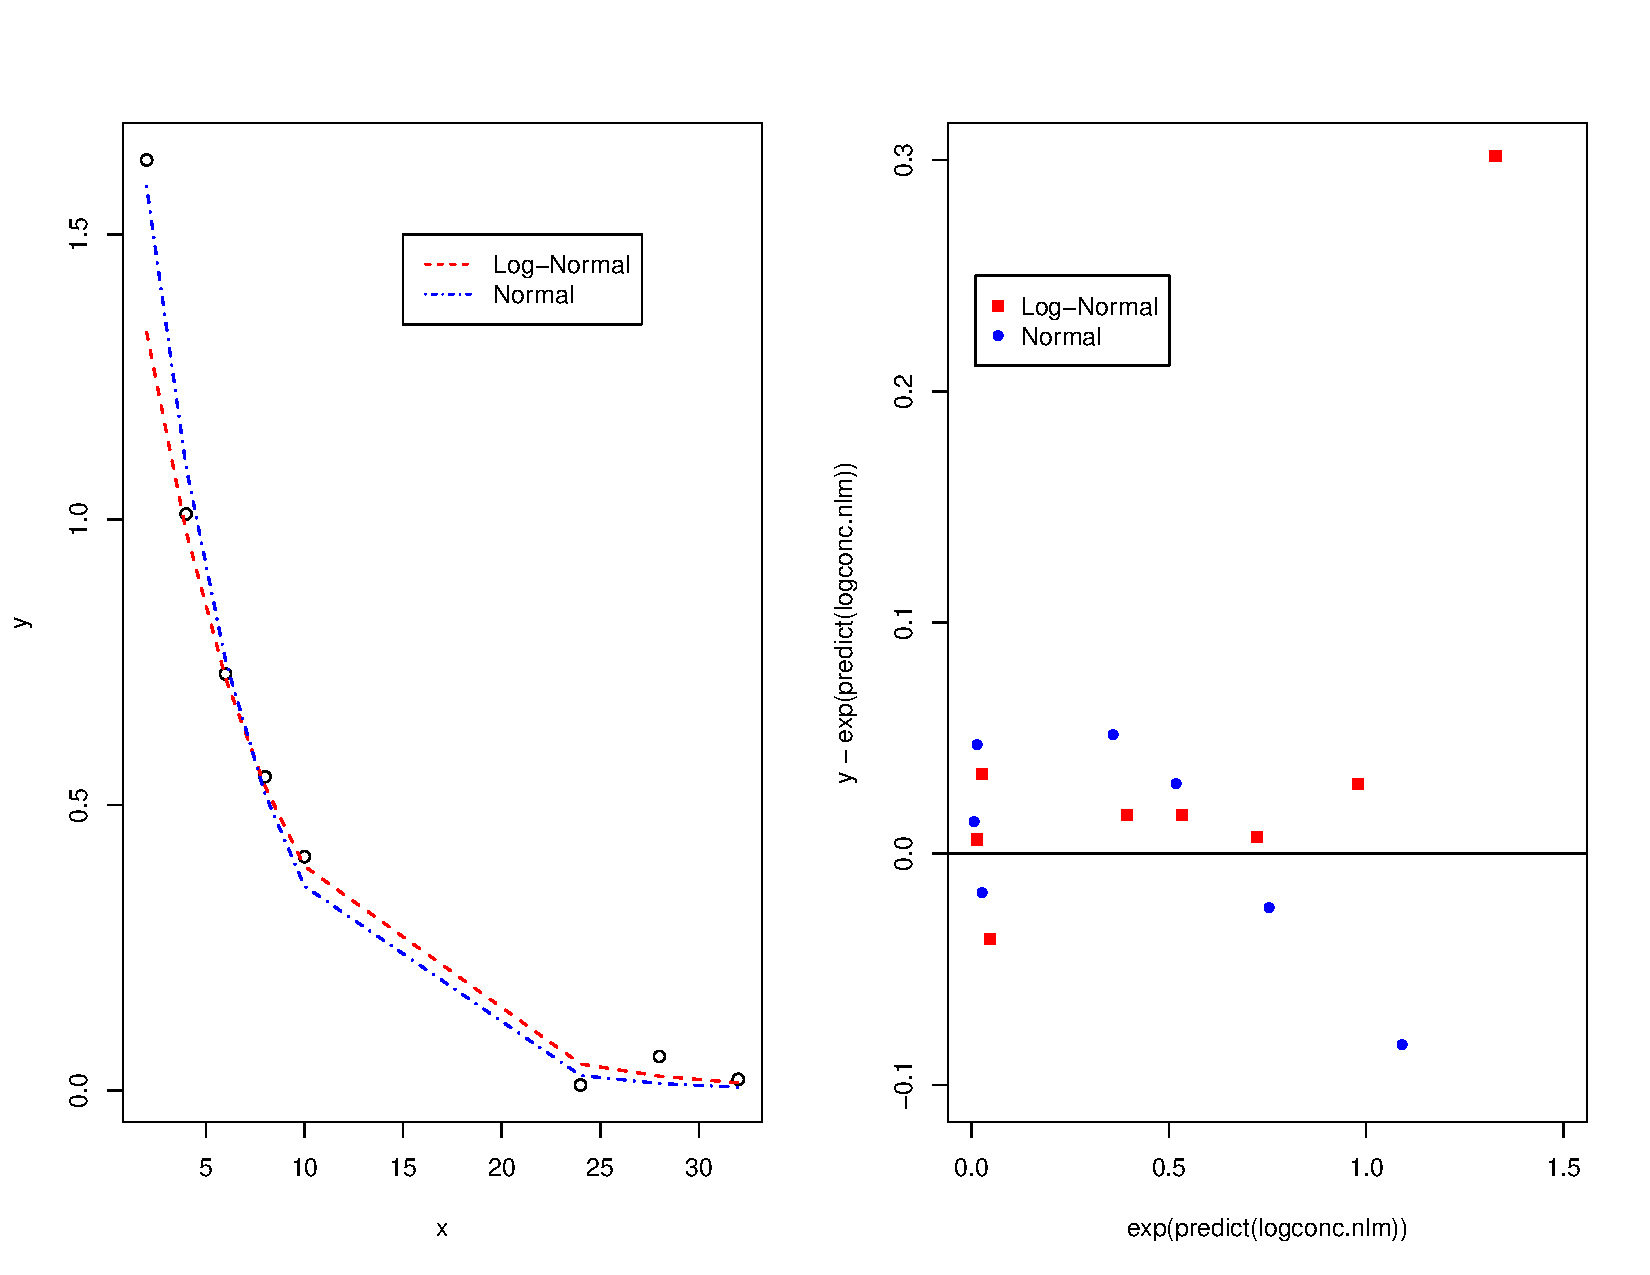
\includegraphics[height=3in]{nonlinear}
\end{frame}

\begin{frame} \frametitle{Functions of Interest}
Interest is in
\begin{itemize}
\item clearance: $V \kappa_e$ \pause
\item elimination half-life $x_{1/2} = \log 2/\kappa_e$ \pause
\end{itemize}

  \begin{itemize}
  \item   Use properties of MLEs: asymptotically  $\hat{\b} \sim N\left(\b,
    I(\hat{\b})^{-1}\right)$ \pause
  \item (Multivariate) Delta Method for transformations  \pause
\item Asymptotic Distributions
  \end{itemize}

Bayes obtain the posterior directly for parameters and functions of parameters!    Priors?  Constraints on Distributions?
\end{frame}

\begin{frame}\frametitle{Summary}
  \begin{itemize}
  \item Optimal transformation for normality (MLE) depends on choice
    of mean function \pause
 \item May not be the same as the variance stabilizing transformation \pause
 \item Nonlinear Models as suggested by Theory or Generalized Linear
   Models are alternatives \pause
 \item ``normal'' estimates may be useful approximations for large $p$
   or for starting values for more complex models  (where convergence
   may be sensitive to starting values)
  \end{itemize}
\end{frame}
\end{document}



